\documentclass[10pt]{article}  

%%%%%%%% PREÁMBULO %%%%%%%%%%%%
\title{Plantilla para reportes de proyecto}
\usepackage[spanish]{babel} %Indica que escribiermos en español
\usepackage[utf8]{inputenc} %Indica qué codificación se está usando ISO-8859-1(latin1)  o utf8  
\usepackage{amsmath} % Comandos extras para matemáticas (cajas para ecuaciones,
% etc)
\usepackage{amssymb} % Simbolos matematicos (por lo tanto)
\usepackage{graphicx} % Incluir imágenes en LaTeX
\usepackage{color} % Para colorear texto
\usepackage{subfigure} % subfiguras
\usepackage{float} %Podemos usar el especificador [H] en las figuras para que se
% queden donde queramos
\usepackage{capt-of} % Permite usar etiquetas fuera de elementos flotantes
% (etiquetas de figuras)
\usepackage{sidecap} % Para poner el texto de las imágenes al lado
	\sidecaptionvpos{figure}{c} % Para que el texto se alinie al centro vertical
\usepackage{caption} % Para poder quitar numeracion de figuras
\usepackage{commath} % funcionalidades extras para diferenciales, integrales,
% etc (\od, \dif, etc)
\usepackage{cancel} % para cancelar expresiones (\cancelto{0}{x})
 
\usepackage{anysize} 					% Para personalizar el ancho de  los márgenes
\marginsize{2cm}{2cm}{2cm}{2cm} % Izquierda, derecha, arriba, abajo

\usepackage{appendix}
\renewcommand{\appendixname}{Apéndices}
\renewcommand{\appendixtocname}{Apéndices}
\renewcommand{\appendixpagename}{Apéndices} 

% Para que las referencias sean hipervínculos a las figuras o ecuaciones y
% aparezcan en color
\usepackage[colorlinks=true,plainpages=true,citecolor=blue,linkcolor=blue]{hyperref}
%\usepackage{hyperref} 
% Para agregar encabezado y pie de página
\usepackage{fancyhdr} 
\pagestyle{fancy}
\fancyhf{}
\fancyhead[L]{\footnotesize UAEH} %encabezado izquierda
\fancyhead[R]{\footnotesize Colegio de posgrado}   % dereecha
\fancyfoot[R]{\footnotesize Sistemas Embebidos}  % Pie derecha
\fancyfoot[C]{\thepage}  % centro
\fancyfoot[L]{\footnotesize Maestría en Internet de las Cosas}  %izquierda
\renewcommand{\footrulewidth}{0.4pt}


\usepackage{listings} % Para usar código fuente
\definecolor{dkgreen}{rgb}{0,0.6,0} % Definimos colores para usar en el código
\definecolor{gray}{rgb}{0.5,0.5,0.5} 
% configuración para el lenguaje que queramos utilizar
\lstset{language=Matlab,
   keywords={break,case,catch,continue,else,elseif,end,for,function,
      global,if,otherwise,persistent,return,switch,try,while},
   basicstyle=\ttfamily,
   keywordstyle=\color{blue},
   commentstyle=\color{red},
   stringstyle=\color{dkgreen},
   numbers=left,
   numberstyle=\tiny\color{gray},
   stepnumber=1,
   numbersep=10pt,
   backgroundcolor=\color{white},
   tabsize=4,
   showspaces=false,
   showstringspaces=false}

\newcommand{\sen}{\operatorname{\sen}}	% Definimos el comando \sen para el seno
%en español

\title{Plantilla de proyecto final}
% Basada en la plantilla para reportes UPIITA de  Overleaf

%%%%%%%% TERMINA PREÁMBULO %%%%%%%%%%%%

\begin{document}

%%%%%%%%%%%%%%%%%%%%%%%%%%%%%%%%%% PORTADA %%%%%%%%%%%%%%%%%%%%%%%%%%%%%%%%%%%%%%%%%%%%
																					%%%
\begin{center}																		%%%
\newcommand{\HRule}{\rule{\linewidth}{0.5mm}}									%%%\left
 																					%%%
\begin{minipage}{0.48\textwidth} \begin{flushleft}

\includegraphics[scale = 0.25]{Imagenes/uaeh.png}
\end{flushleft}\end{minipage}
\begin{minipage}{0.48\textwidth} \begin{flushright}

\includegraphics[scale = 0.25]{Imagenes/colpos2.png}
\end{flushright}\end{minipage}

													 								%%%
\vspace*{1.0cm}								%%%
																					%%%	
\textsc{\huge Universidad Autónoma del Estado de\\ \vspace{5px}Hidalgo}\\[1.5cm]	

\textsc{\LARGE Colegio de Posgrado }\\[1.5cm]													%%%

\begin{minipage}{0.9\textwidth} 
\begin{center}																					%%%
\textsc{\LARGE Sistemas Embebidos }
\end{center}
\end{minipage}\\[0.5cm]
%%%
    																				%%%
 			\vspace*{1cm}																		%%%
																					%%%
\HRule \\[0.4cm]																	%%%
{ \huge \bfseries Implementación de modelo de referencia IoT de Cómputo en el borde sobre Computadora mono-placa (SBC) Orange Pi 5 Plus y nodo inteligente en Sistema mono-chip (SoC) ESP32 }\\[0.4cm]	%%%
 																					%%%
\HRule \\[1.5cm]																	%%%
 																				%%%
																					%%%
\begin{minipage}{0.46\textwidth}													%%%
\begin{flushleft} \large															%%%

% Aqui a continuación pongan los nombres de los integrantes
\emph{Nombre del alumno:}\\	
I.S.C. Erick Renato Vega Ceron \\

%%%
			%\vspace*{2cm}	
            													%%%
										 						%%%
\end{flushleft}																		%%%
\end{minipage}		
																%%%
\begin{minipage}{0.52\textwidth}		
\vspace{-0.6cm}											%%%
\begin{flushright} \large															%%%
\emph{Profesor:} \\																	%%%
Dr. Ismael Domínguez Jiménez.\\
													%%%
\end{flushright}																	%%%
\end{minipage}	
\vspace*{1cm}
%\begin{flushleft}
 	
%\end{flushleft}
%%%
 		% \flushleft{\textbf{\Large Nombre del curso (IMEC XXZZ)}	}\\																		%%%
\vspace{2cm} 																				
\begin{center}	
Torre de posgrado - Ciudad del Conocimiento \\
{\large \today}																	%%%
 			\end{center}												  						
\end{center}							 											
																					
\newpage																		
%%%%%%%%%%%%%%%%%%%% TERMINA PORTADA %%%%%%%%%%%%%%%%%%%%%%%%%%%%%%%%

\tableofcontents 

\newpage

\section{Resumen.}

En el contexto de un mundo hipercomunicado en el que la mayoría de los habitantes de las zonas urbanas cuentan con un dispositivo de comunicación inteligente ''Smartphone'', se presenta la oportunidad de aprovechar la tecnología de telecomunicaciones digitales subyacente en el fomento a ciudades más inteligentes, inclusivas y sostenibles. 

En el marco de los 17 objetivos de desarrollo sostenible establecidos por la Organización de las Naciones Unidas, la movilidad urbana forma parte del desarrollo de Ciudades y Comunidades más sostenibles. La operación, gestión y eficiencia del sistema de transporte público presenta desafíos significativos que son parte de las tareas de los operadores del transporte.La falta de coordinación y comunicación causan la degradación del servicio. La tecnología informática del Internet de las Cosas permite el desarrollo de aplicaciones que ayuden en la solución de tales desafíos. 

En el siguiente artículo se estudia la implementación del modelo de referencia IoT a casos de uso comunes al transporte público en la ciudad de Pachuca de Soto, Hidalgo, iniciando con el desarrollo y pruebas de prototipo inicial.
\cite{IEEEreferencias:Ref1}
\cite{IEEEreferencias:Ref2}



\section{Introducción.} 

El proyecto ``Cahuitl'' implementa tecnologías de Internet de las Cosas en hardware embebido.
El sistema recolecta datos de nodos sensores inteligentes que luego se transmiten a una Computadora de Placa Única (SBC) para el procesamiento y la presentación en redes locales y remotas, la comunicación es bidireccional, lo que permite controlar actuadores remotamente. 


\section{Problema a resolver}

Según datos del INEGI, en 2015, de los 557,093 habitantes aproximados en la Zona Metropolitana de Pachuca, alrededor de 67,874 personas trabajan o estudian en otro municipio, dependiendo del transporte público para desplazarse a sus lugares correspondientes. En la actualidad, los usuarios del transporte público en la ZMP enfrentan largos tiempos de espera y desconocen por completo las rutas disponibles. Además, los conductores deben encargarse del cobro de pasajes, la gestión de tiempos de ruta y la conducción del vehículo, lo que afecta la calidad del servicio, aumenta el riesgo de un percance y disminuye la adopción del transporte público, agravando la problemática. 
\cite{IEEEreferencias:Ref3}

\section{Propuesta de Solución}
Para abordar estos desafíos, la gestión de rutas, el cobro automatizado y la recolección de datos operativos se destacan como soluciones clave. Ejemplo de estas implementaciones son los casos en Ciudad de México o Guadalajara, donde el cobro automatizado y la gestión de rutas ya se han implementado en el transporte masivo. 

La implementación de tecnologías que optimicen las rutas, reduzcan los tiempos de espera, simplifiquen los pagos y mejoren la certeza del servicio para los usuarios puede revitalizar la confianza en el transporte público. La recopilación y análisis de datos permiten una toma de decisiones más informada, contribuyendo así a un sistema de transporte más eficiente y atractivo para los viajeros.\cite{IEEEreferencias:Ref4}\cite{IEEEreferencias:Ref5}
\section{Objetivo}
Este proyecto tiene como objetivo desarrollar el prototipo de un sistema de cobro automatizado basado en tecnología LoRa que mejore la experiencia del pasajero. El desarrollo del mismo sigue una metodología de desarrollo evolutiva que permitirá realizar pruebas en la distancia, el retardo en las señales y el ancho de banda necesario para una comunicación entre dispositivos para distintos casos de uso.


\subsection{Objetivos Específicos}

\begin{enumerate}


\item Objetivo 1 - Desarrollar un nodo de sensores inteligente basado en un Sistema Monochip (SoC) que permita recolectar datos de un sensor de temperatura y humedad (DHT11) y un dispositivo de posicionamiento global (GPS), realizar un procesamiento local de la información obtenida basado en rangos predefinidos y transmitir la información a un periférico de salida que permita mostrar texto. 

\item Objetivo 2 - Transmitir datos del nodo sensor entre conductor y cliente utilizando tecnología WiFi de corto alcance bajo el protocolo de red MQTT ligero y emitirlos a una computadora mono-placa, la cual deberá procesar los datos recibidos, almacenarlos y presentarlos gráficamente en un panel de control en la red local utilizando el protocolo HTTP. Transmitir los datos a un servidor en la nube para su presentación en línea.

\item Objetivo 3 - Permitir el control de actuadores en el nodo inteligente (dispositivo usuario) y en el nodo de control (dispositivo conductor) por medio de un panel de control en la red local. 
\end{enumerate}


\section{Material a utilizar}
Para el desarrollo del proyecto se utilizarán los siguientes componentes:
   \begin{enumerate}
    \item Microcontrolador ESP32 DevKitC: Sistema en un Chip (SoC) con optimizaciones para el prototipado
    \item Sensor DHT11: Sensor digital de temperatura y humedad de alta precisión y estabilidad.
    \item Pantalla OLED 128x64: Dispositivo periférico de salida para presentación de texto  
    \item Placa de prototipado LK32 para fácil acceso a GPIO
    \item Orange Pi 5 Plus: Computadora mono-placa con sistema operativo Orange OS basado en Arch Linux
    \item Relevador de 5V: Relevador srd-05vdc-sl-c utilizado ampliamente en electrónica para la conmutación de cargas de corriente
    \item Servomotor SG90: Servomotor de bajo torque para actuación mecánica 
   \end{enumerate}

\section{Implementación de prototipo}

El proyecto se desarrolló modularmente en el marco de la Maestría en Internet de las Cosas, desarrollando diversos módulos y pruebas de concepto de las diferentes tecnologías en las materias Sistemas Embebidos, Introducción al Internet de las Cosas y Redes de Comunicaciones en el semestre junio-diciembre de 2023.

El modelo de referencia utilizado para la implementación del Internet de las Cosas permite segmentar las distintas tecnologías, protocolos, etapas de procesamiento y flujo de datos a lo largo del ciclo de vida de la aplicación; de esta manera, es posible definir un paradigma de arquitectura que cubra el flujo desde los dispositivos de borde, el ''Edge Computing'', pasando por dispositivos encargados del almacenamiento, análisis y transformación de los datos medidos en los nodos sensores inferiores, estos aparatos son conocidos también como "cómputo de niebla", hasta las capas superiores que permiten desplegar aplicaciones individuales y servicios en la nube sobre servidores en internet. 
\cite{IEEEreferencias:Ref6}
\begin{figure}[H]
	\begin{center}
	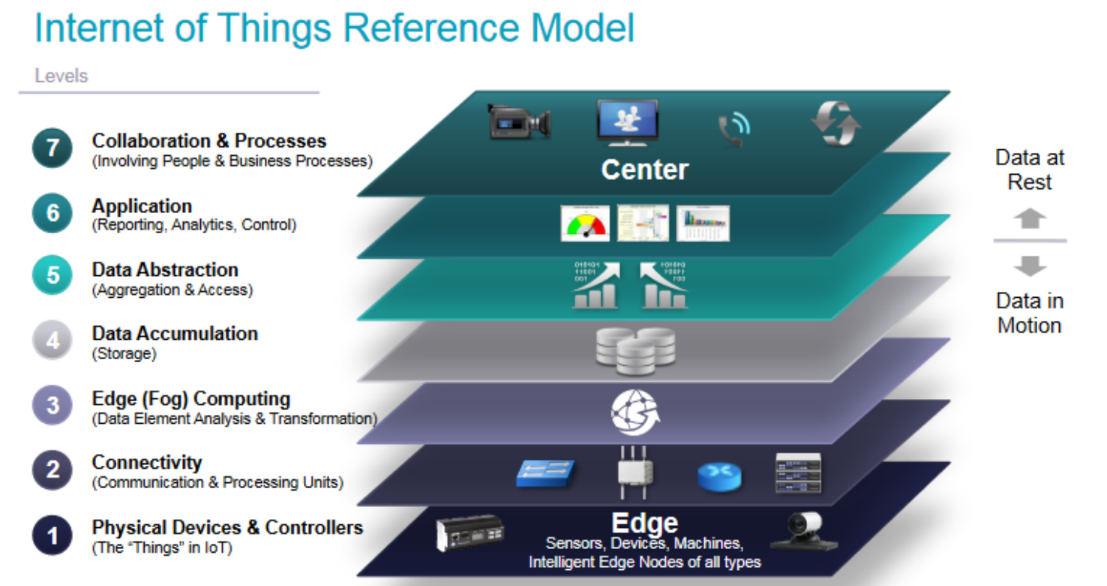
\includegraphics[scale=0.5]{Imagenes/modeloreferencia.png} 
 		\captionof{figure}{\label{fig:modeloreferencia}Modelo de referencia para Internet de las Cosas (Cisco, 2014)} 
	\end{center} 
\end{figure}

Al inicio del proyecto, se utilizó la placa de expansión Laika LK32 fabricada en México por Hola Laika. Esta placa incluye componentes de hardware embebidos para simplificar las conexiones y la gestión de la energía suministrada al microcontrolador ESP32-DevKitC y la regulación eléctrica necesaria para trabajar a valores de voltaje entre los 3 a 6 volts, suficiente para satisfacer los requisitos de alimentación de los sensores y actuadores, del nodo inteligente ''Dispositivo Pasajero''. 
\cite{IEEEreferencias:Ref7}
\begin{figure}[H]
	\begin{center}
	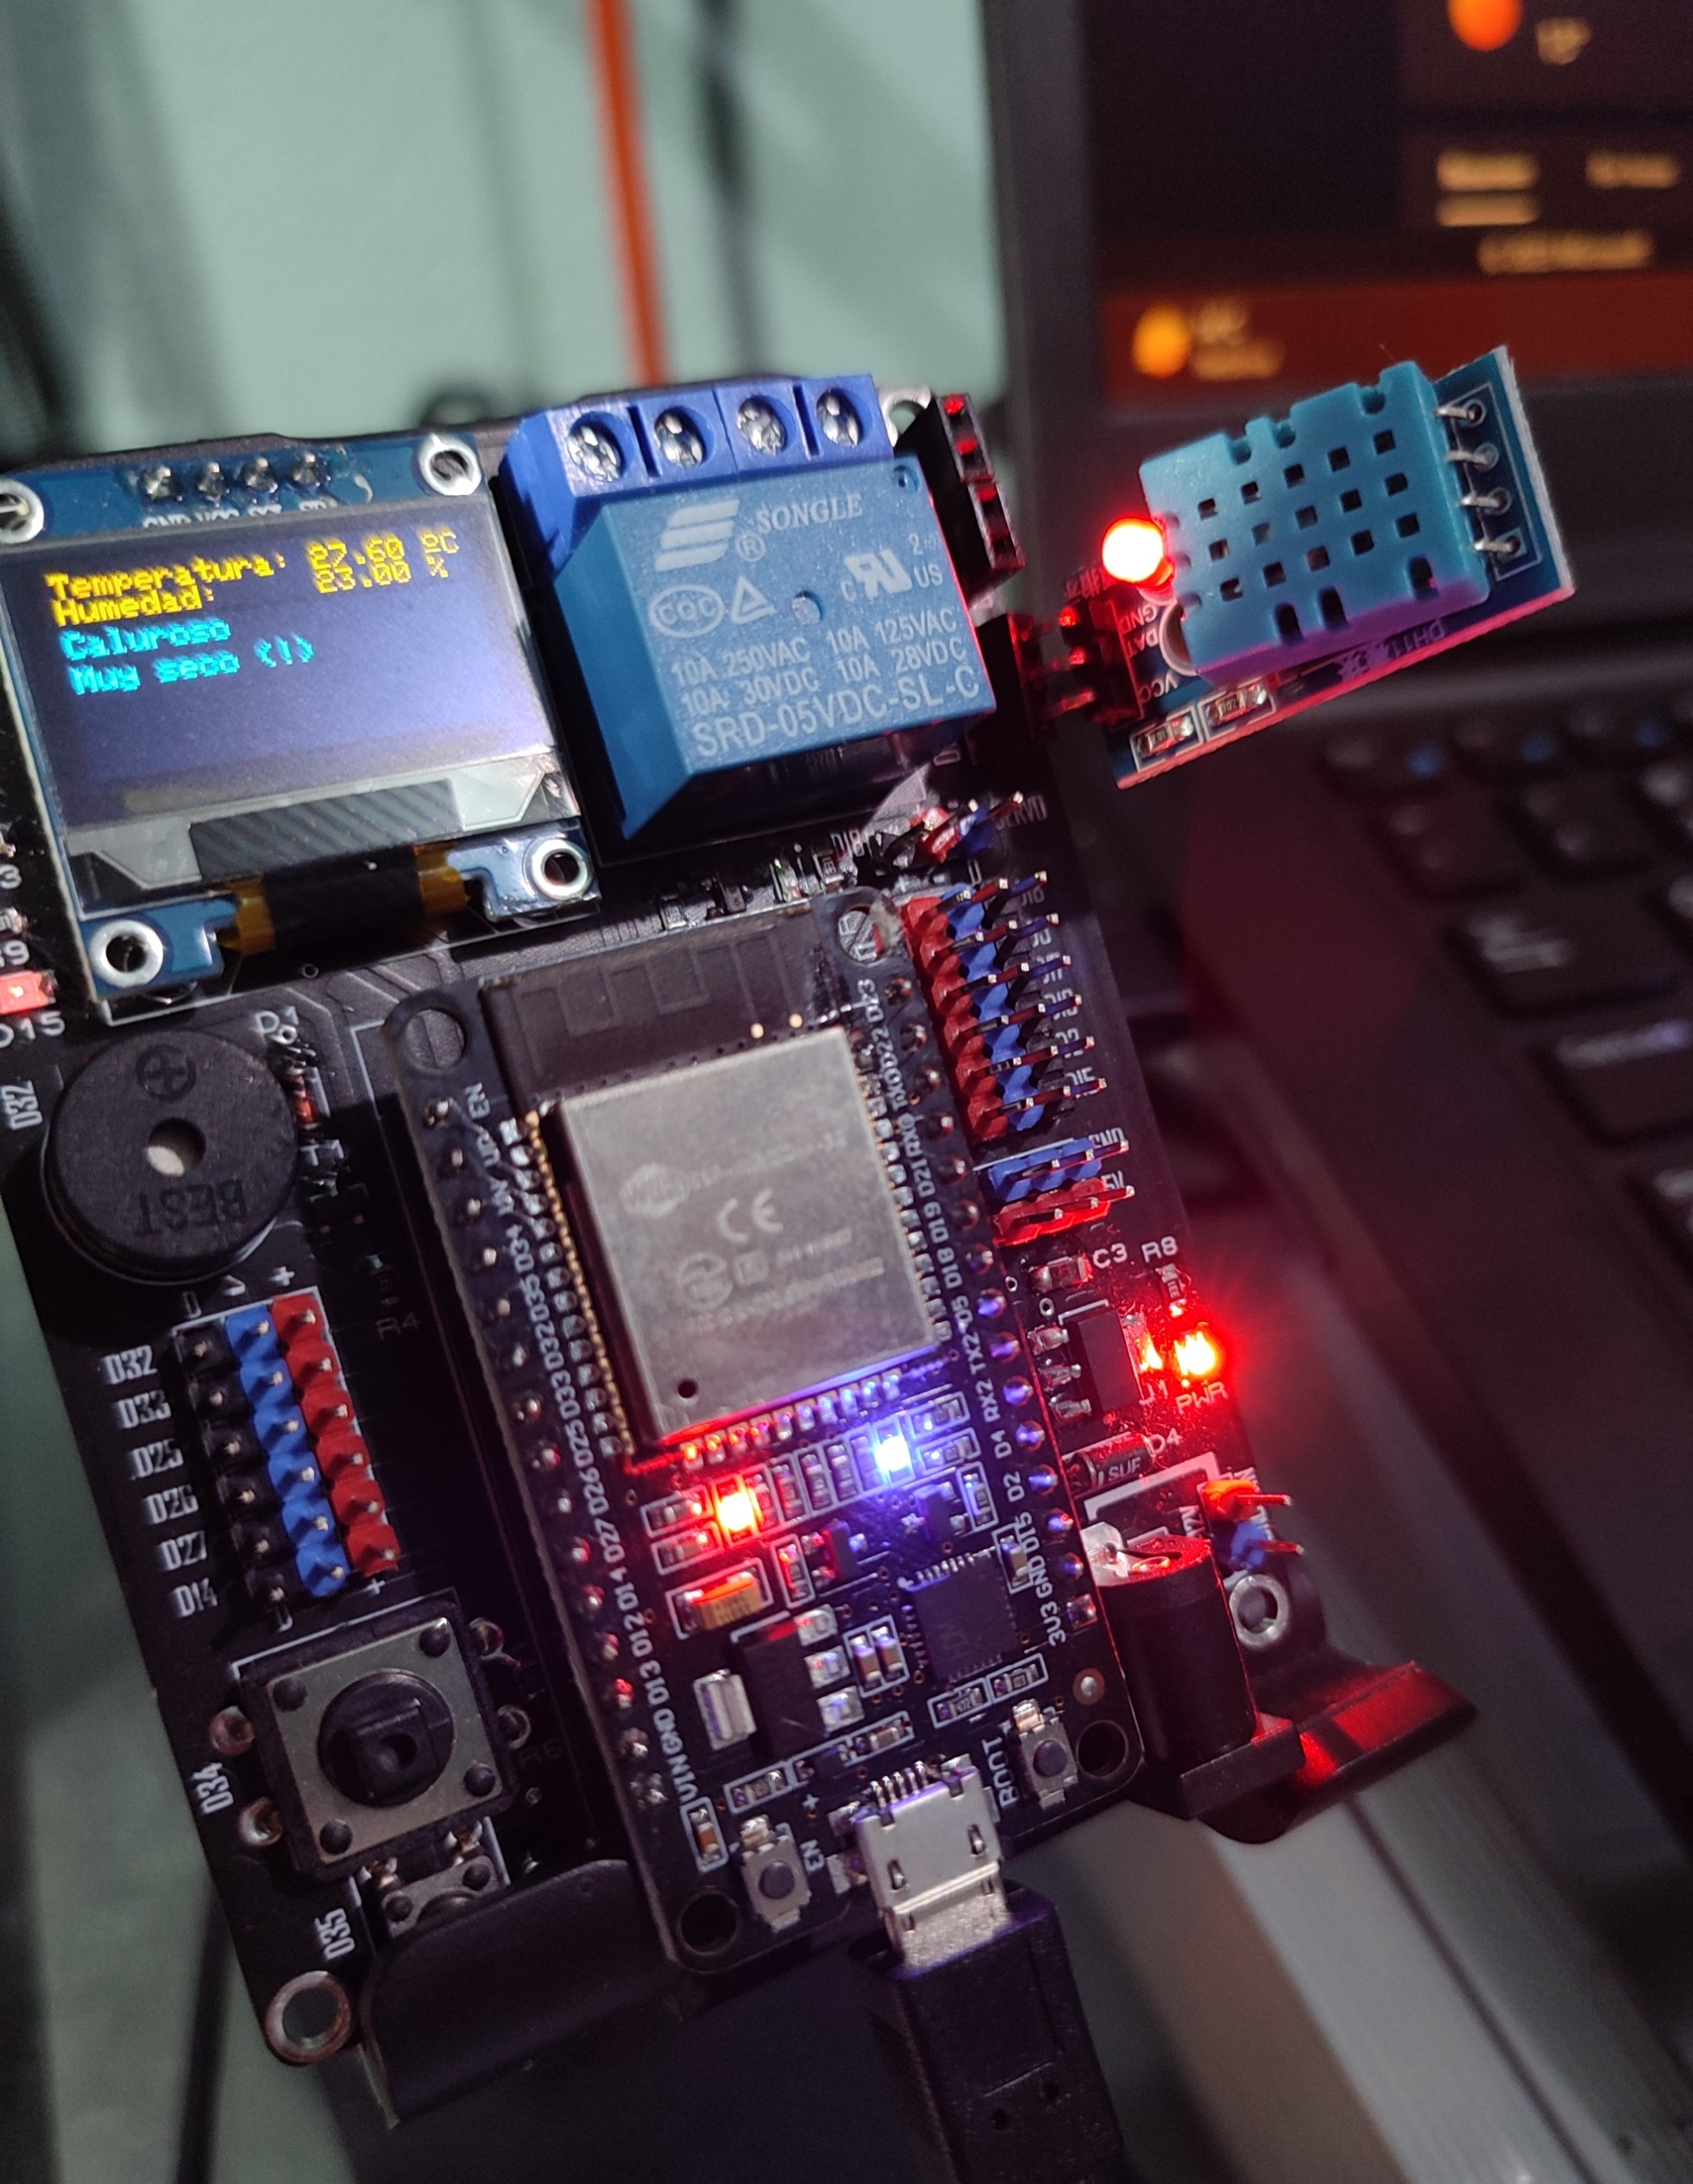
\includegraphics[scale=0.1]{Imagenes/lk32_sensores.png} 
 		\captionof{figure}{\label{fig:lk32_sensores}Placa LK32} 
	\end{center} 
\end{figure}
El código utilizado para el nodo de sensores se puede encontrar en el repositorio del proyecto:
\href{https://github.com/Dtcsrni/Cahuitl}{Repositorio de Proyecto Cahuitl}.
\cite{IEEEreferencias:Ref8}
El software utilizado para controlar al sensor inteligente basado en el ESP32 implementa librerías del entorno Arduino para el control de los sensores DHT11 y GPS.
\begin{figure}[H]
	\begin{center}
	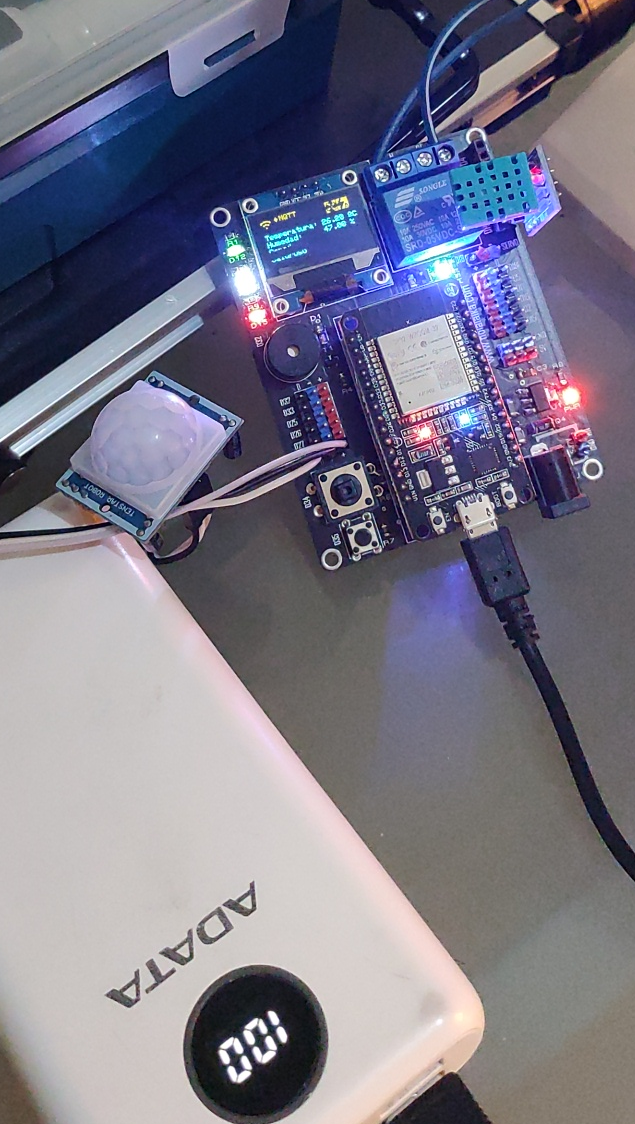
\includegraphics[scale=0.3]{Imagenes/sensor_powerbank.png} 
 		\captionof{figure}{\label{fig:sensor_powerbank}Módulo sensor inteligente con un sensor PIR y un banco de poder de 20mil mAh} 
	\end{center} 
\end{figure}
Una vez realizadas las pruebas con el sensor de humedad y temperatura, se procedió a probar la conexión con el módulo Neo-6M para obtener las coordenadas del dispositivo y calibrar el timestamp recibido para sincronizarse a la zona horaria local (GMT -6)
\begin{figure}[H]
	\begin{center}
	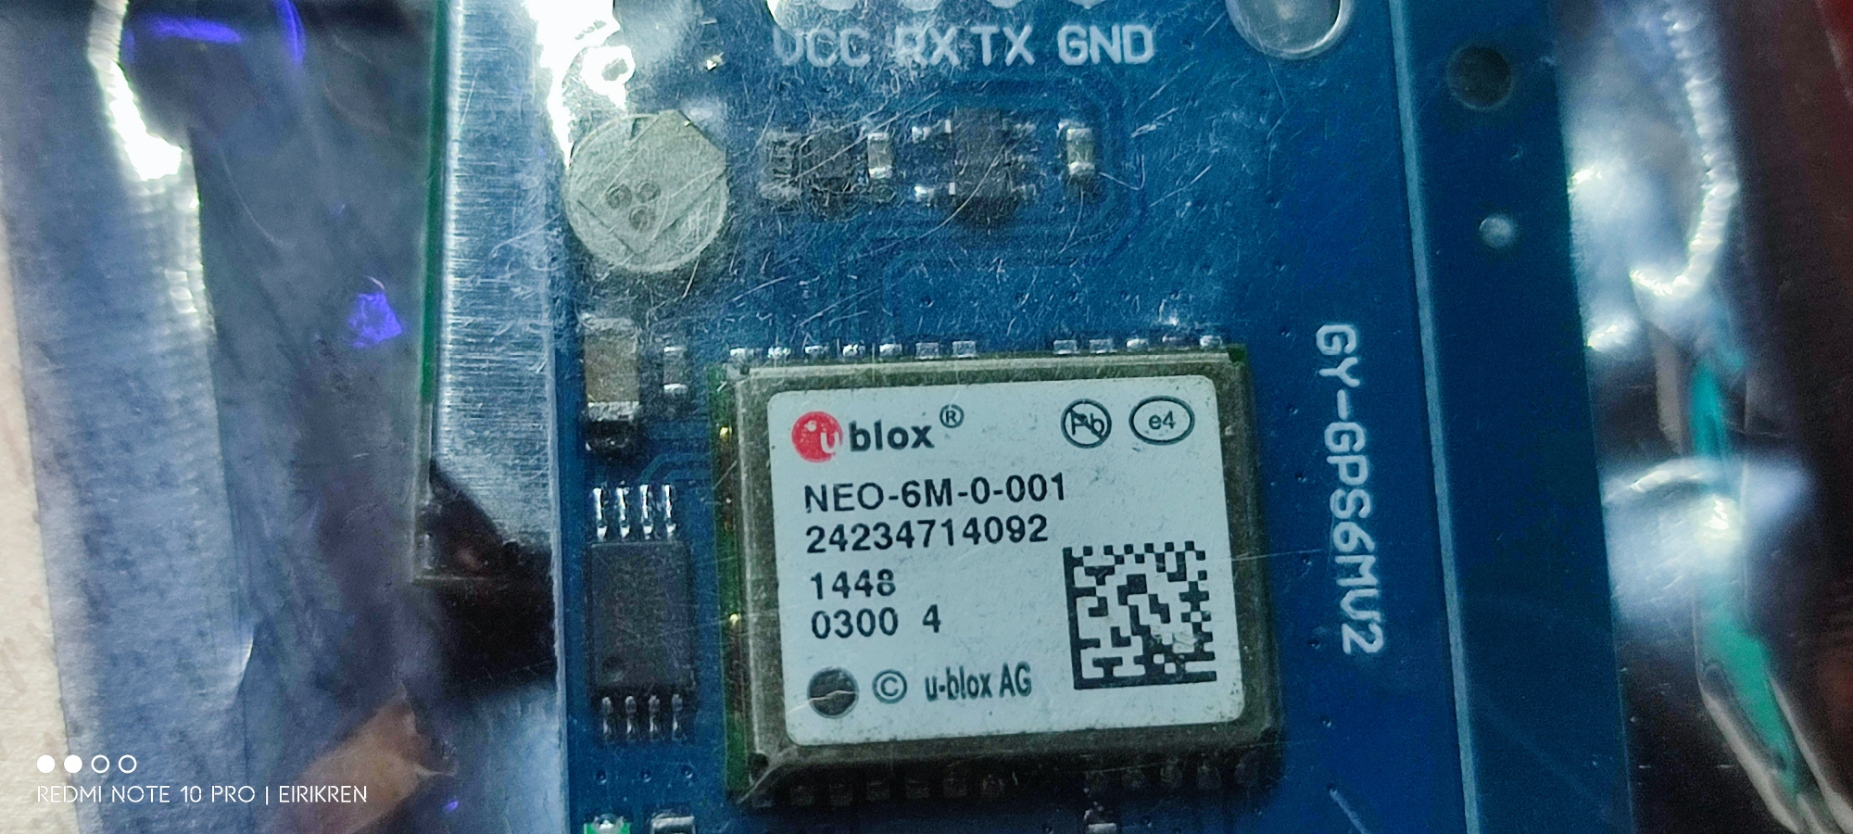
\includegraphics[scale=0.3]{Imagenes/neo-6m.png} 
 		\captionof{figure}{\label{fig:neo-6m}Módulo GPS Neo-6M en formato de desarrollo con pines soldados} 
	\end{center} 
\end{figure}
\begin{figure}[H]
	\begin{center}
 		\includegraphics[width = 0.5\textwidth]{Imagenes/cahuitl.png}
 		\captionof{figure}{\label{fig:cahuitl}Nodo sensor inteligente con los módulos GPS, DHT11 y PIR contectados, alimentado por powerbank} 
	\end{center} 
\end{figure}
\begin{figure}[H]
	\begin{center}
 		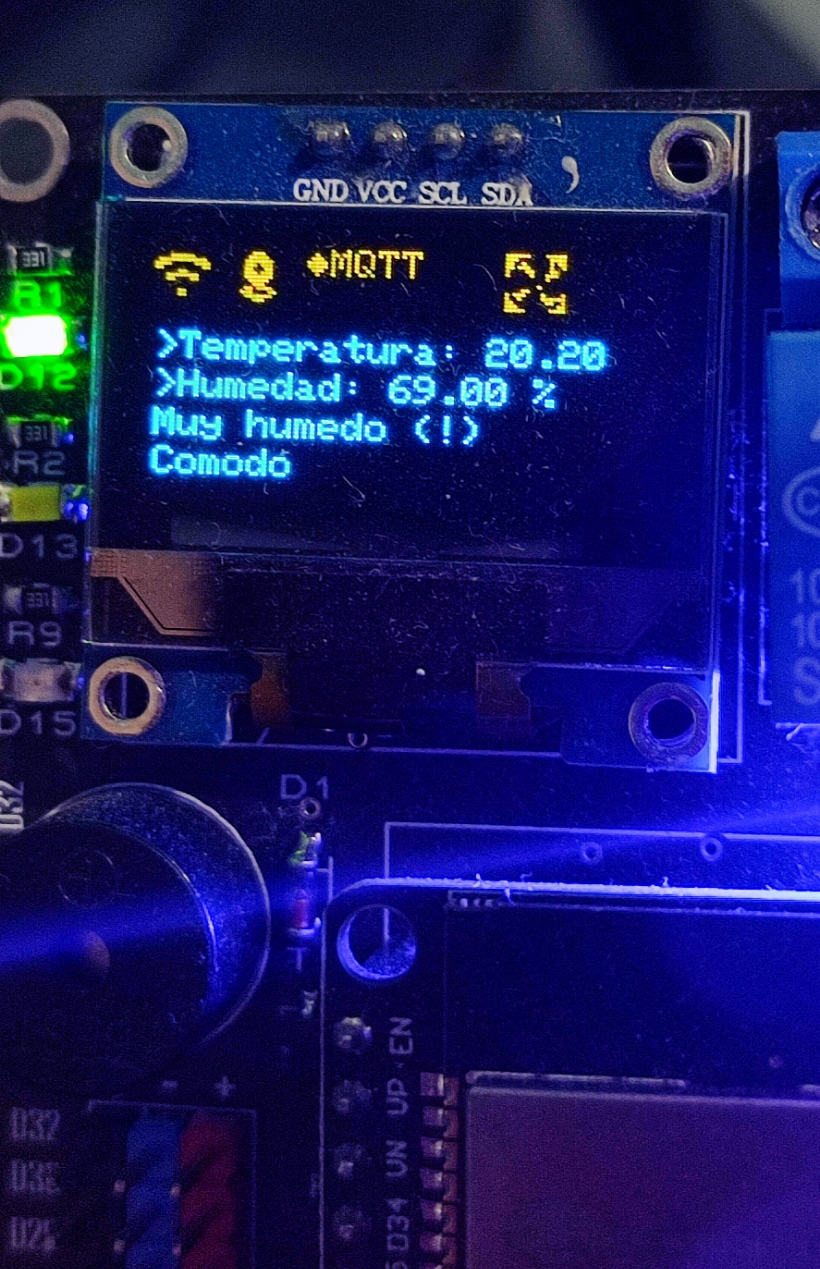
\includegraphics[width = 0.5\textwidth]{Imagenes/oled128x64.png}
 		\captionof{figure}{\label{fig:oled128x64}Detalle de pantalla OLED 128x64 Adafruit SSD1306 mostrando algunos íconos informativos del estado del nodo, datos de los sensores y análisis de ambiente} 
	\end{center} 
\end{figure}

Para simplificar la gestión de datos se utilizó la herramienta web Node-Red, la cual permite manejar por medio de un sistema de nodos los diferentes componentes de hardware y software en un sistema de IoT. El flujo implementado para el proyecto es el siguiente:
\begin{figure}[H]
	\begin{center}
 		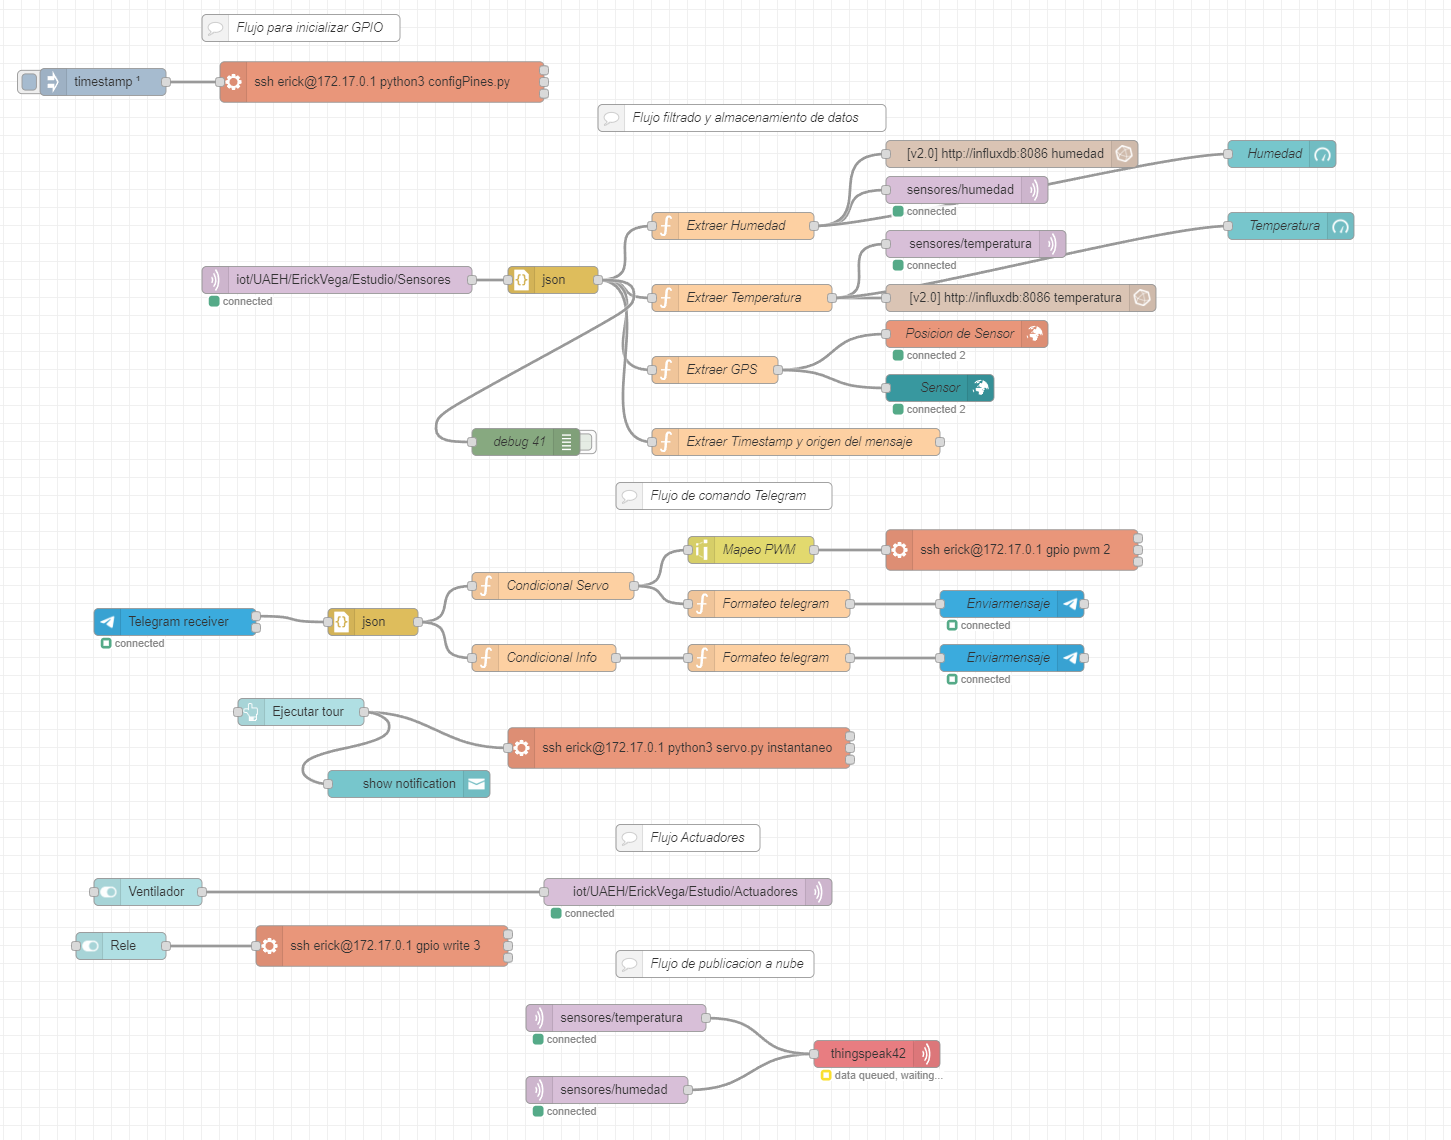
\includegraphics[width = 1\textwidth]{Imagenes/nodosCahuitl.png}
 		\captionof{figure}{\label{fig:nodosCahuitl}Flujo de proyecto Cahuitl} 
	\end{center} 
\end{figure}
En dicho flujo se implementaron las siguientes funciones:
 \begin{enumerate}
    \item Inicialización de puertos GPIO en SBC Orange Pi 5 Plus
    \item Monitoreo de paquetes MQTT desde el nodo inteligente de sensores y descomposición en magnitudes de medición
    \item Geolocalización de coordenadas emitidas por módulo GPS y presentación sobre mapas en panel de control
    \item Control de servomotor por medio de señales PWM a GPIO de SBC Orange Pi 5 Plus utilizando la aplicación de mensajería instantánea Telegram
    \item Envío de estado de nodo inteligente de sensores y sus mediciones bajo demanda utilizando Telegram
    \item Implementación de tour de servomotor por medio de scripts de Python ejecutados sobre sistema operativo Linux Orange Pi 5 Plus
    \item  Control de ventilador por medio de uso de relevador utilizando elementos gráficos de interfaz de usuario en el panel principal de Node-Red
    \item  Envío de paquetes con datos de sensores a plataforma ThingSpeak para presentación de datos en línea
     \end{enumerate}
Para reducir la necesidad de mantenimiento de los componentes individuales de software utilizados, se ha implementado la plataforma de contenedores de software abierto Docker.De esta manera, se puede crear un ecosistema interconectado basado en sistemas distribuidos sobre una arquitectura de virtualización ligera sobre un ecosistema heterogéneo de hardware (nodos inteligentes).
\cite{IEEEreferencias:Ref9}
\begin{figure}[H]
	\begin{center}
 		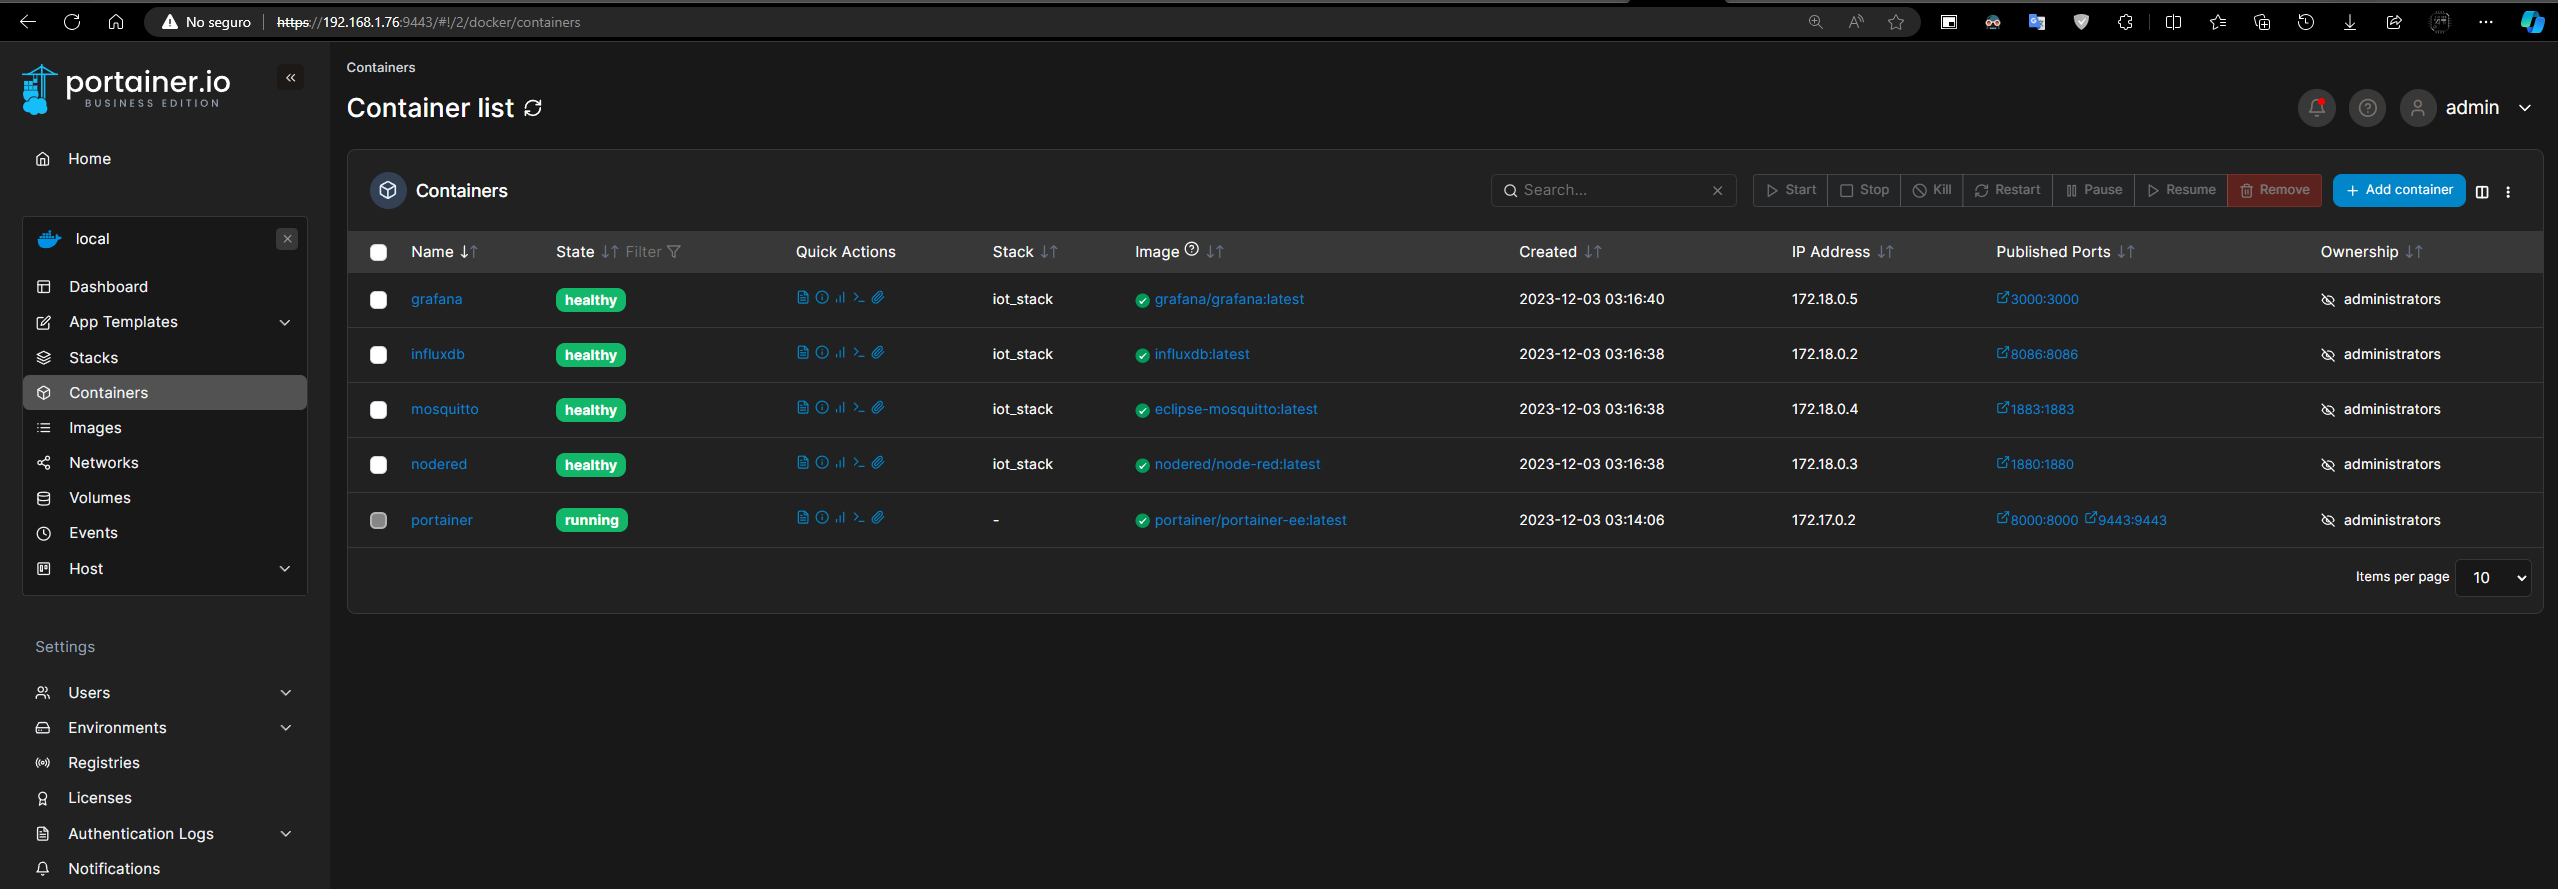
\includegraphics[width = 1\textwidth]{Imagenes/portainer.png}
 		\captionof{figure}{\label{fig:contenedoresPortainer}Contenedores desplegados sobre panel de monitoreo Portainer} 
	\end{center} 
\end{figure}

Los datos recopilados así como los controles que forman parte del Panel de control principal se despliegan por medio del uso de ''dashboards'' de la herramienta Node-Red. El software de Node-Red, Grafana (Generación de gráficos con base en datos recopilados), Mosquitto (Protocolo MQTT de mensajería ligera), InfluxDB (Capa de persistencia de datos) y Portainer (monitoreo de contenedores) se despliegan sobre el sistema operativo Orange OS, una distribución de Arch Linux para arquitecturas de computadoras ARM de 64 bits (Aarch64) proporcionado por el fabricante de la SBC (Single Board Computer) Orange Pi 5 Plus fabricada en China por Shenzhen Xunlong Software Co.
\cite{IEEEreferencias:Ref10}
\begin{figure}[H]
	\begin{center}
 		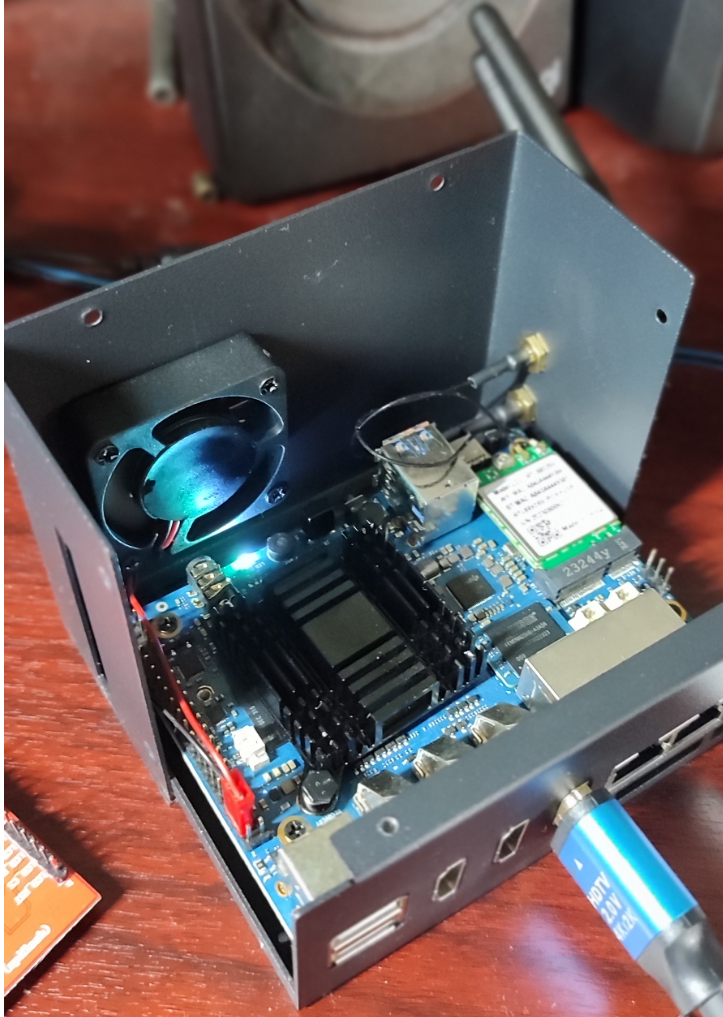
\includegraphics[width = 0.5\textwidth]{Imagenes/orangepi5p.png}
 		\captionof{figure}{\label{fig:orangepi5p} SBC (Single Board Computer) Orange Pi 5 Plus montada sobre un estuche metálico. En la figura se aprecia el módulo Wifi/Bluetooth que habilita la conectividad inalámbrica, un disipador de temperatura sobre el SoC, un pequeño ventilador de 5 volts y las antenas para mejorar la calidad de las señales emitidas y recibidas por la capa física de red} 
	\end{center} 
\end{figure}
\begin{figure}[H]
	\begin{center}
 		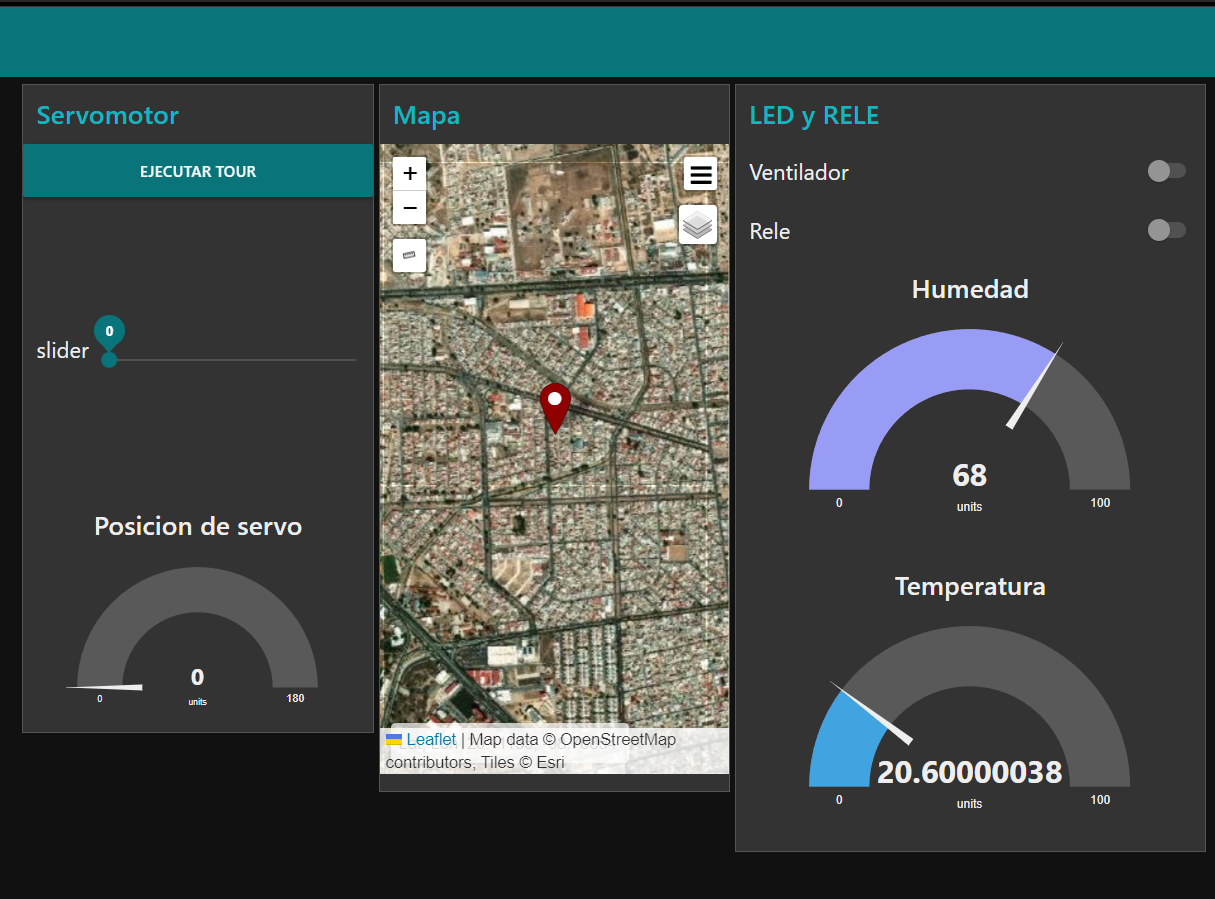
\includegraphics[width = 0.5\textwidth]{Imagenes/panelControl.png}
 		\captionof{figure}{\label{fig:panelControl} Panel de Control Principal sobre la aplicación HTTP Node-Red. En la imagen se aprecia un mapa con la localización del módulo GPS, controles de posición y 'tour' del servomotor, activadores del relevador que conecta un ventilador de 120 volts en el nodo inteligente y un relevador en el GPIO del SBC así como gráficos que indican el estado de los sensores. } 
	\end{center} 
\end{figure}
Los contenedores se encuentran así en un ecosistema más escalable y eficiente, que se beneficia de la arquitectura ARM de bajo consumo de la SBC. 


\subsection{Diagrama a bloques}
El siguiente diagrama de bloques permite visualizar los diferentes componentes del sistema embebido, así como las interacciones entre dispositivos y redes
\begin{figure}[H]
	\begin{center}
 		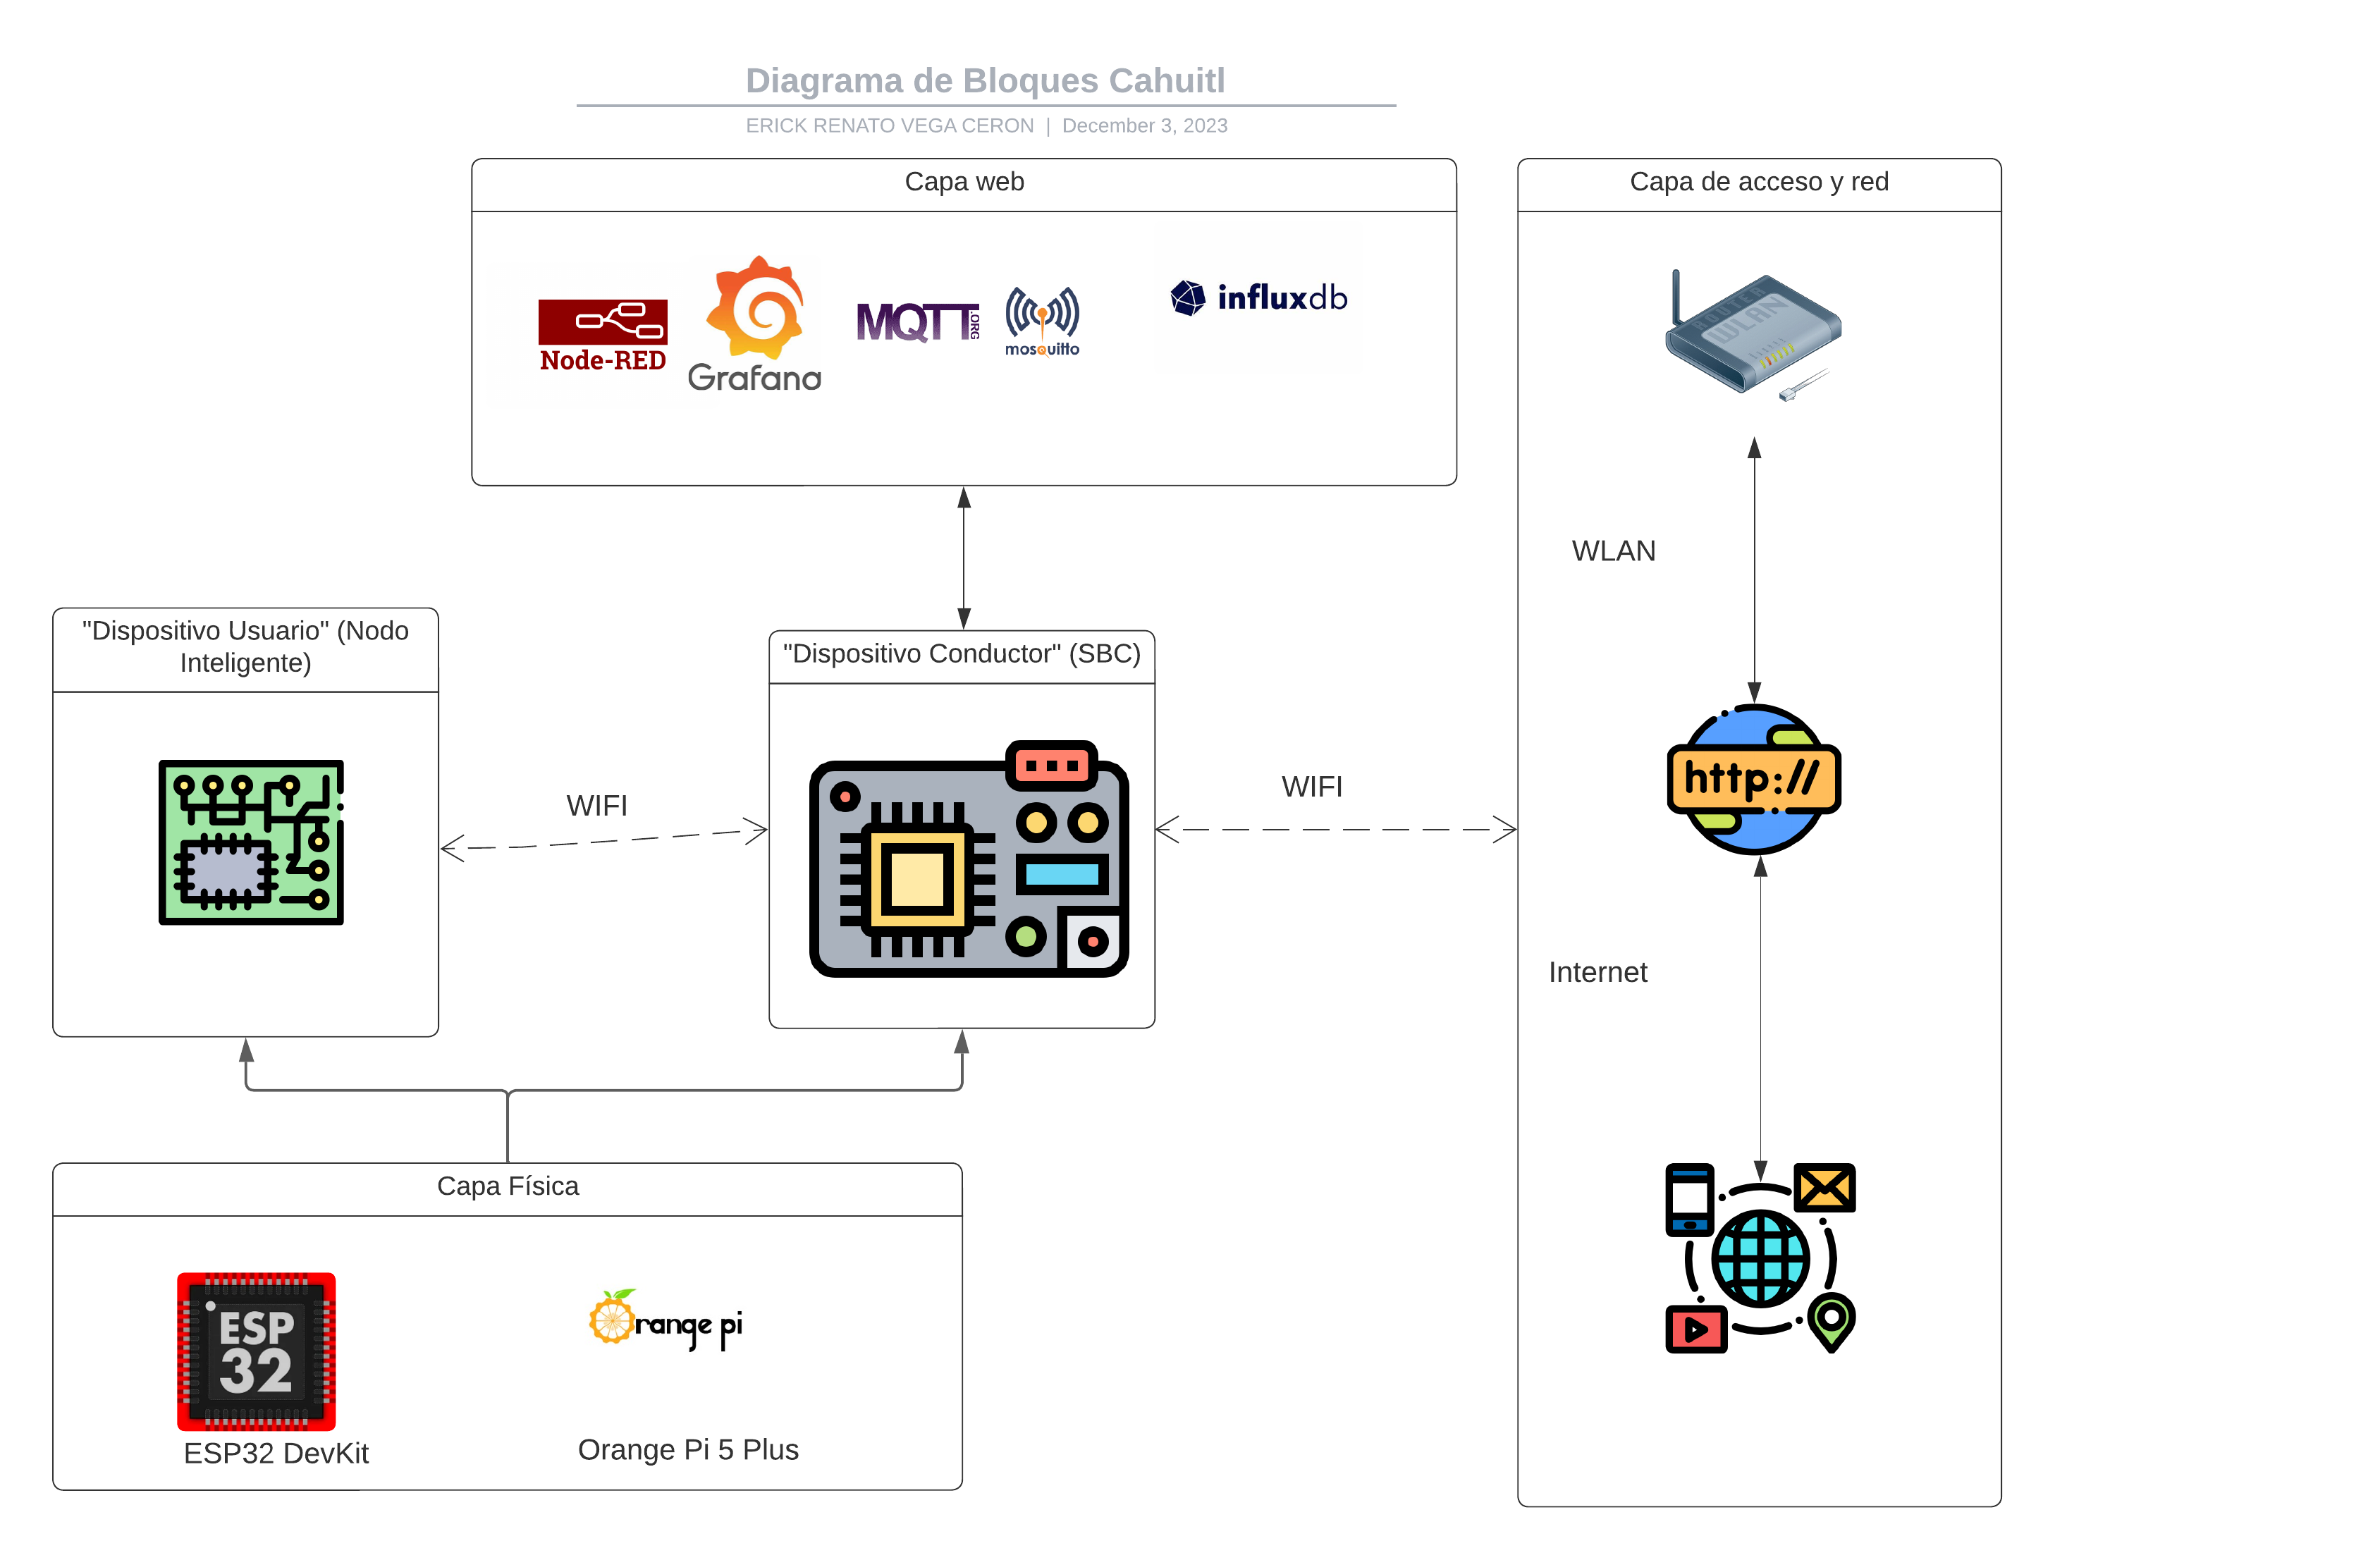
\includegraphics[width = 1\textwidth]{Imagenes/diagramaBloques.png}
 		\captionof{figure}{\label{fig:diagramaBloques}Diagrama de bloques del sistema Cahuitl} 
	\end{center} 
\end{figure}



\section{Conclusiones.}

El prototipo Cahuitl implementa eficientemente un ''stack'' de tecnologías del Internet de las Cosas sobre un sistema de hardware embebido como prueba de concepto que en el futuro permitirá adaptar el diseño presentado a las necesidades de una plataforma de automatización de transporte público. 
En futuras iteraciones se plantea la implementación de sensores RFID para la lectura de tarjetas, así como un periférico de salida en el dispositivo conductor que permita ofrecer consejos de ruta e información relevante con base en la analítica realizada en el SBC y los datos de control centralizados en la nube. 

\begin{figure}[H]
	\begin{center}
 		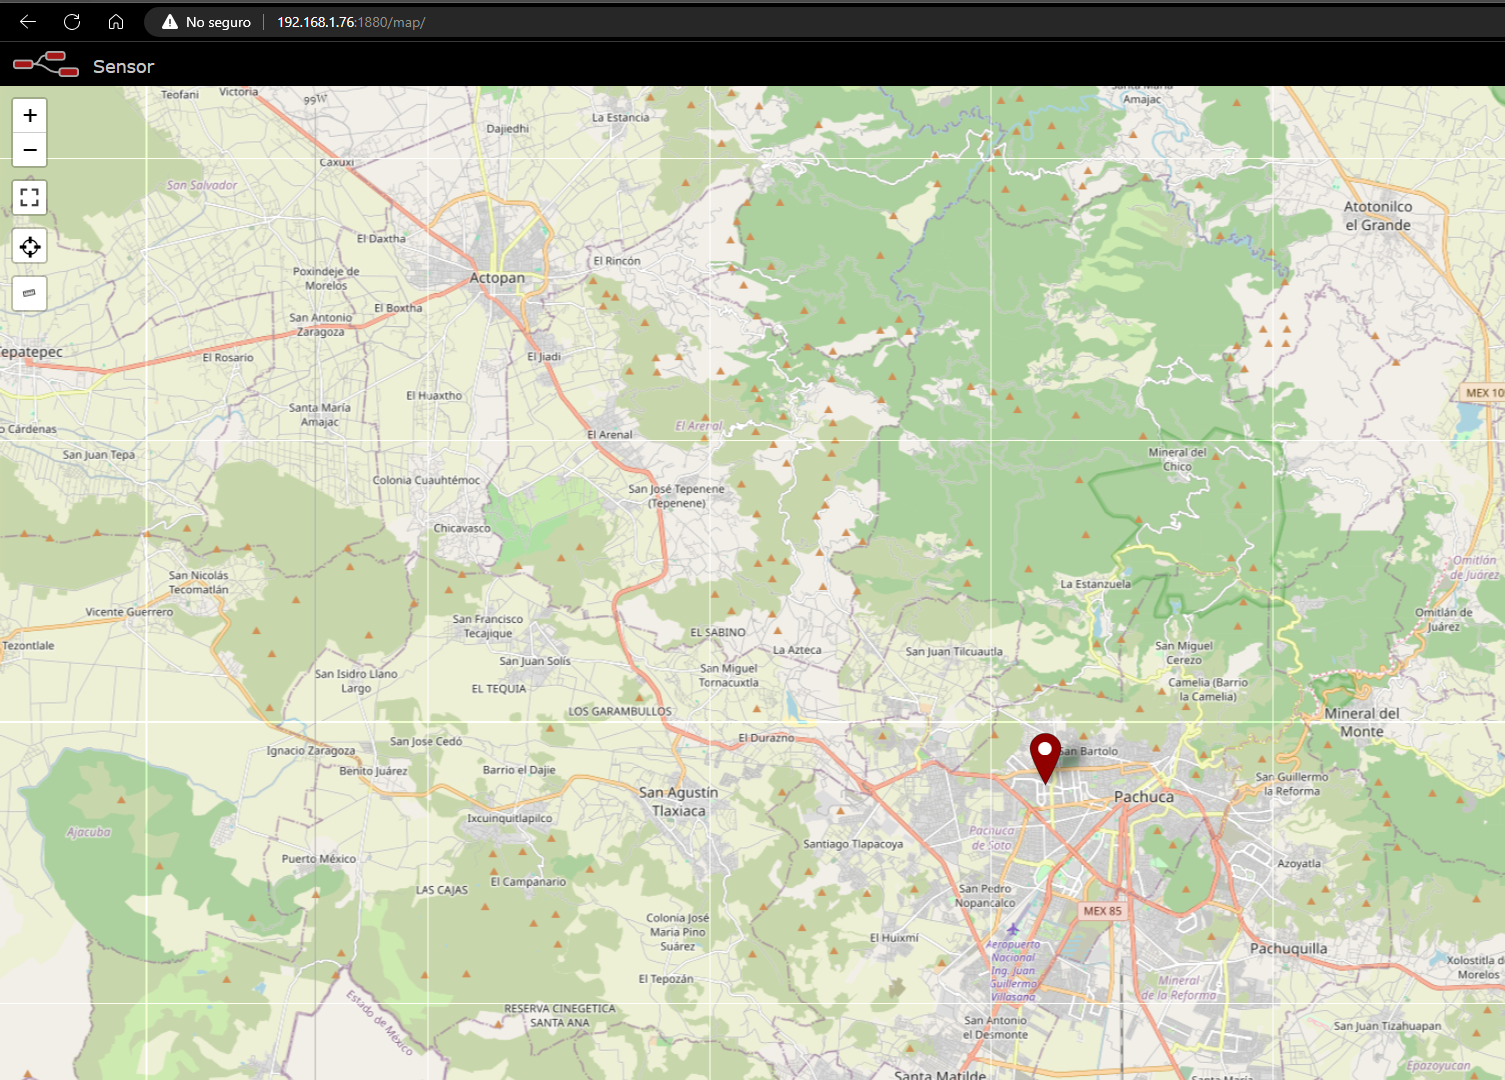
\includegraphics[width = 0.9\textwidth]{Imagenes/mapaGPS.png}
 		\captionof{figure}{\label{fig:mapaGPS}Mapa de geolocalización del sensor GPS en el Nodo Inteligente} 
	\end{center} 
\end{figure}
\begin{figure}[H]
	\begin{center}
 		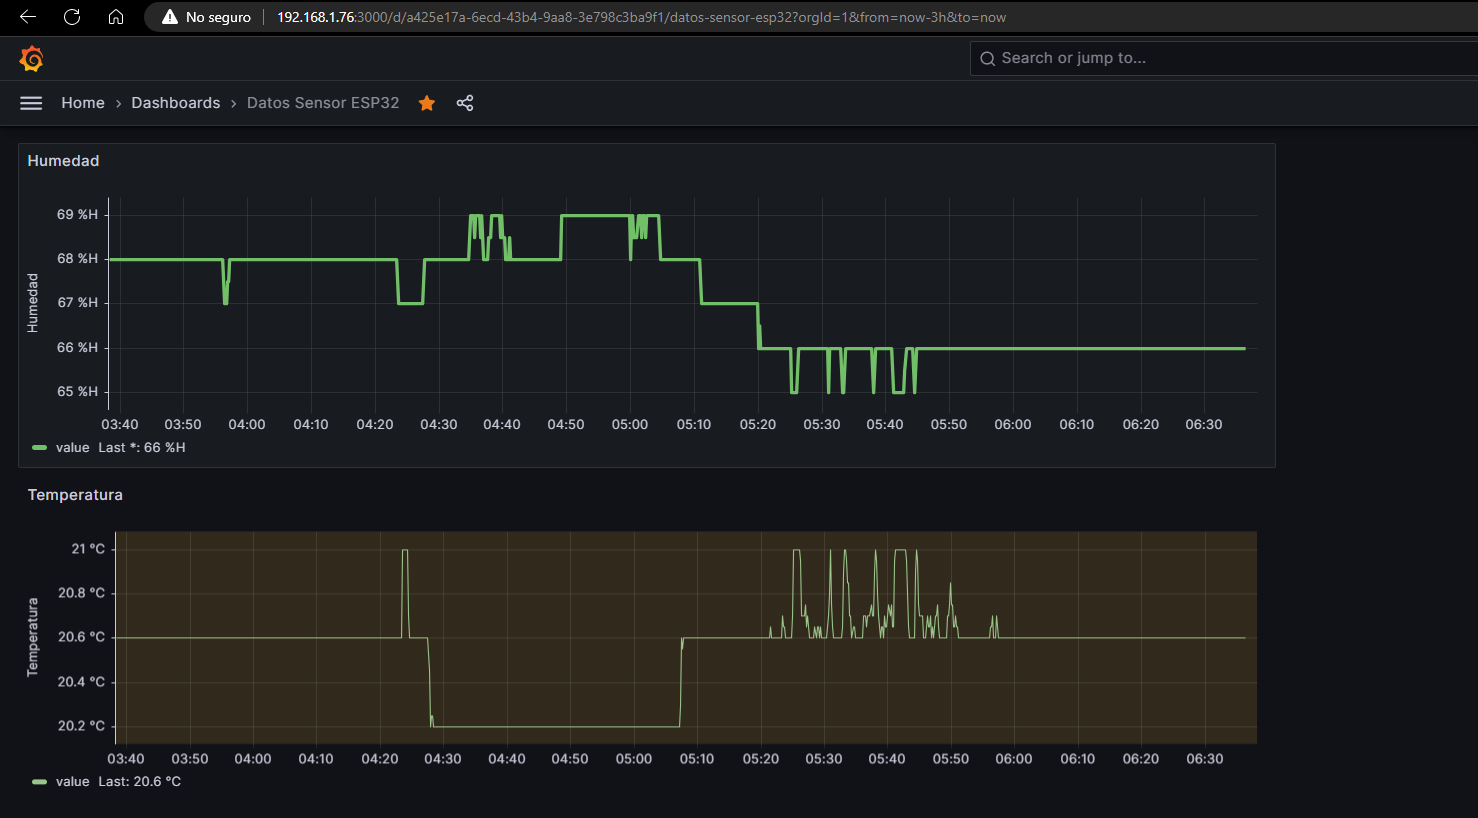
\includegraphics[width = 0.9\textwidth]{Imagenes/grafana.png}
 		\captionof{figure}{\label{fig:grafana}Herramienta de visualización de datos recolectados por Nodo Inteligente Grafana} 
	\end{center} 
\end{figure}
\begin{figure}[H]
	\begin{center}
 		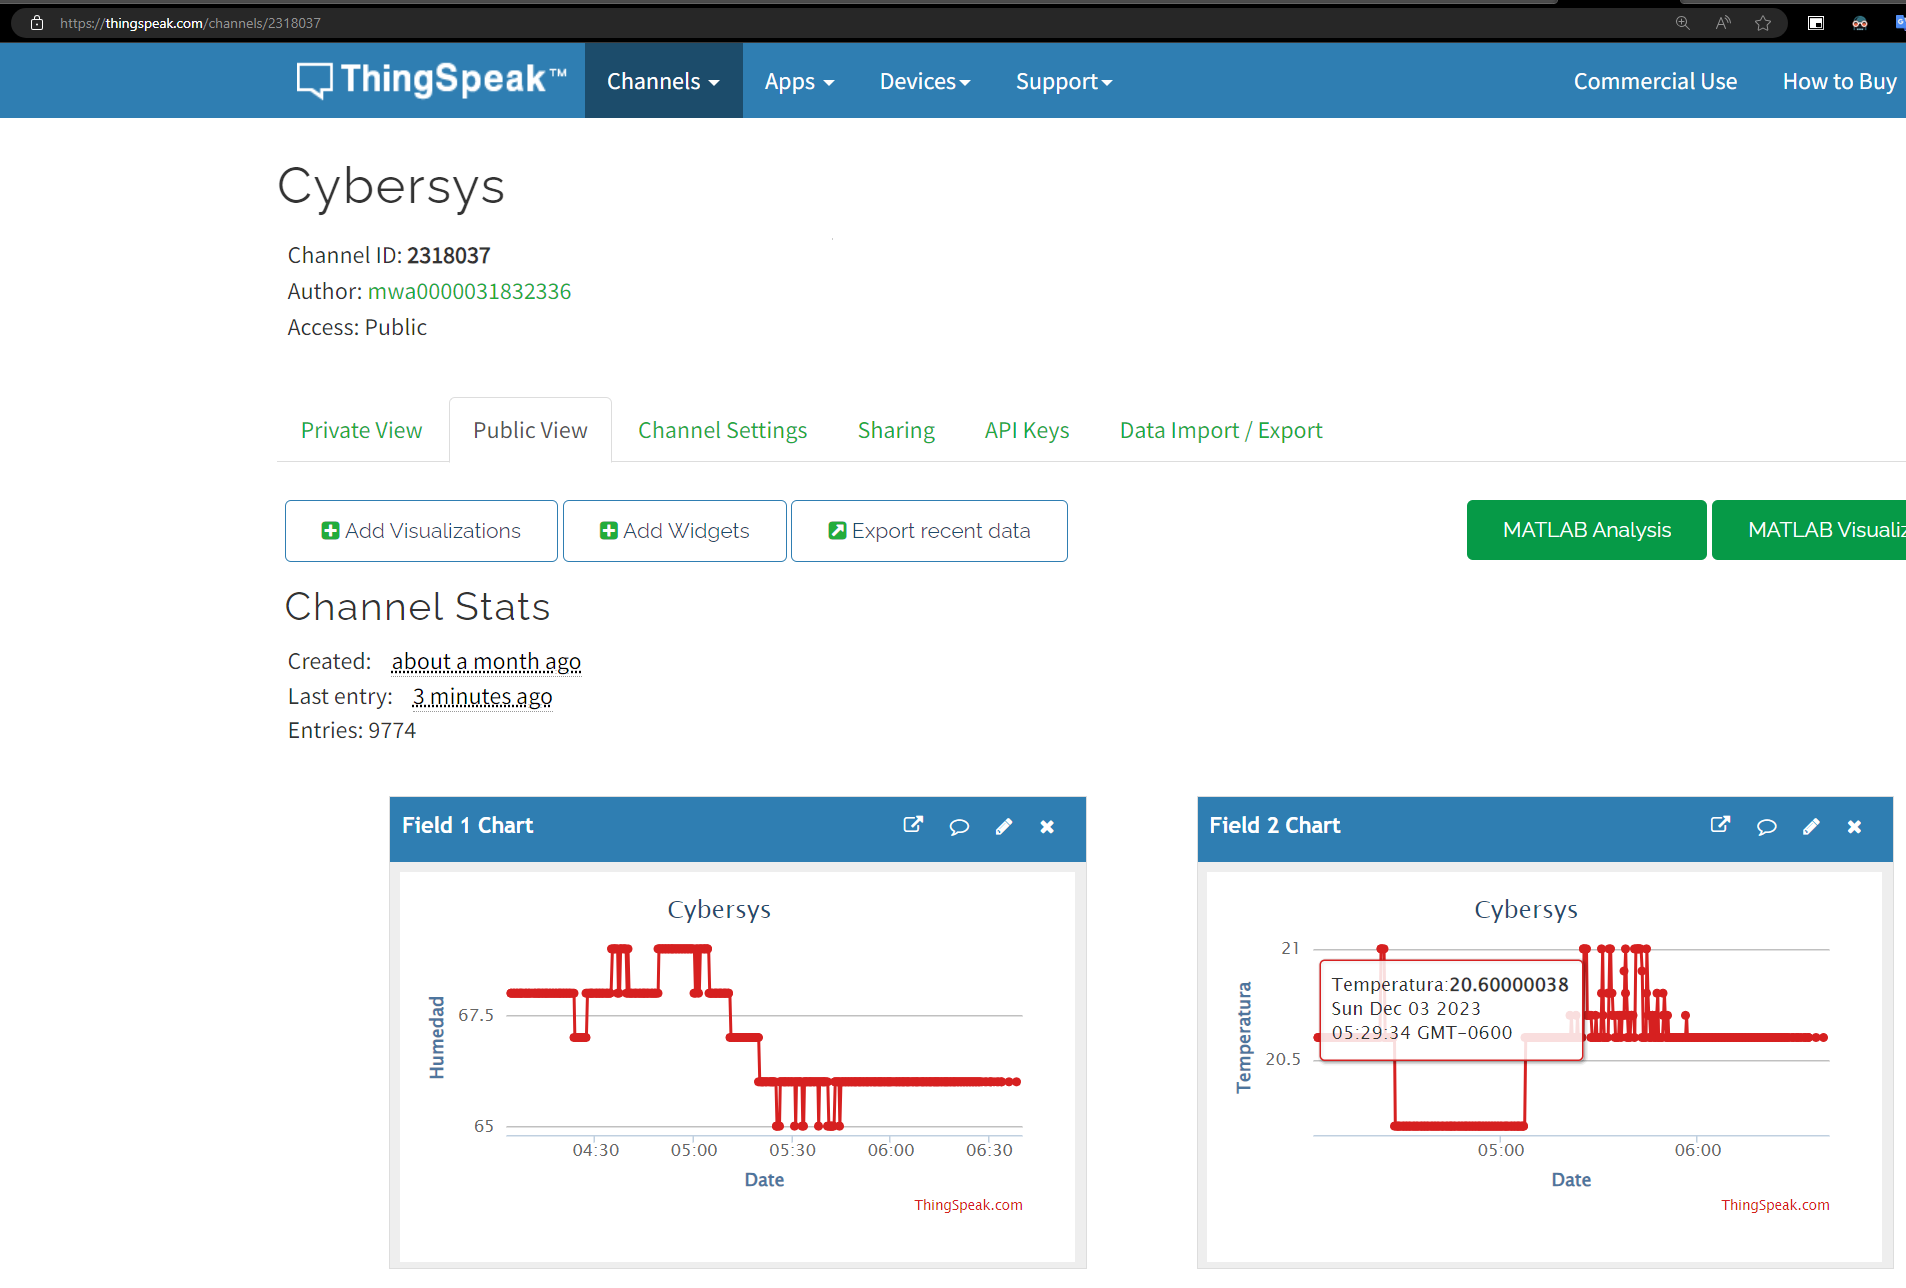
\includegraphics[width = 0.9\textwidth]{Imagenes/thingspeak.png}
 		\captionof{figure}{\label{fig:thingspeak}Panel de visualización de datos de sensor inteligente en nube pública IoT ThingSpeak} 
	\end{center} 
\end{figure}

Como se aprecia en las imágenes, es posible visualizar grandes conjuntos de datos precisos almacenados en la SBC, lo cual permitiría aplicar políticas de actuadores basadas en contexto para la implementacion, monitoreo y adaptación inteligente de rutas de transporte público. La implementación de sensores inteligentes en el transporte público permitirá aportar al desarrollo de proyectos sobre ''Ciudades Inteligentes'' que mejoren la sustentabilidad urbana de tales asentamientos humanos.
\cite{IEEEreferencias:Ref11}

%%%%%%% Bibliografía %%%%%%%%
\bibliographystyle{bst/IEEEtran.bst} 
\addcontentsline{toc}{section}{Referencias}  
\bibliography{bib/IEEEreferencias.bib} 
%%%%%%% Bibliografía %%%%%%%%    



\end{document}